\documentclass[aspectratio=169,10pt]{beamer}
\usepackage{tikz}
\usepackage[scaled=.92]{helvet}
\renewcommand{\familydefault}{\sfdefault}
\usetikzlibrary{positioning,arrows.meta,calc}
\definecolor{bg}{HTML}{071014}
\definecolor{panel}{HTML}{101D22}
\definecolor{active}{HTML}{16262C}
\definecolor{line}{HTML}{2A3D43}
\definecolor{text}{HTML}{E8F0F1}
\definecolor{muted}{HTML}{8AA0A5}
\definecolor{green}{HTML}{69D69A}
\definecolor{mint}{HTML}{A4F0C3}
\definecolor{amber}{HTML}{E8B85E}
\definecolor{red}{HTML}{EC746D}
\definecolor{blue}{HTML}{78B8DB}
\setbeamercolor{background canvas}{bg=bg}
\setbeamercolor{normal text}{fg=text,bg=bg}
\setbeamercolor{frametitle}{fg=text,bg=bg}
\setbeamercolor{block title}{fg=text,bg=active}
\setbeamercolor{block body}{fg=text,bg=panel}
\setbeamertemplate{blocks}[rounded][shadow=false]
\setbeamertemplate{navigation symbols}{}
\setbeamersize{text margin left=7mm,text margin right=7mm}
\setbeamerfont{frametitle}{size=\LARGE,series=\bfseries}
\setbeamerfont{block title}{series=\bfseries}
\setbeamertemplate{itemize item}{\color{mint}$\blacktriangleright$}
\setbeamertemplate{footline}{\hfill{\color{muted}\scriptsize HELIOS -- HOW THE SYSTEM WORKS \quad \insertframenumber/\inserttotalframenumber\hspace{6mm}\vspace{3mm}}}
\newcommand{\status}[2]{\textcolor{#1}{\scriptsize\bfseries #2}}
\newcommand{\tagcurrent}{\status{green}{CURRENT}}
\newcommand{\tagdev}{\status{amber}{IN DEVELOPMENT}}
\newcommand{\tagplanned}{\status{blue}{PLANNED}}
\begin{document}

\begin{frame}[plain]
\begin{tikzpicture}[remember picture,overlay]
  \fill[blue,opacity=.05] (13,2.5) circle (3.6);
  \draw[blue,opacity=.18,line width=18pt] (13,2.5) circle (2.3);
  \draw[green,opacity=.24,line width=4pt] (13,2.5) circle (3.2);
  \draw[mint,opacity=.38,line width=1.1pt] (9.8,5.6)--(15.8,.5);
\end{tikzpicture}
\vspace{9mm}{\color{mint}\Large\bfseries HELIOS}\par\vfill
{\color{text}\fontsize{30}{34}\selectfont\bfseries How the System Works}\par\vspace{3mm}
{\color{text}\Large Operational world, Cortex, Missions, robotic assets, and resilient Site cells}\par\vspace{8mm}
{\color{blue}\large CONTROLLED TECHNICAL OVERVIEW}\par\vfill
{\color{muted}\small Architecture and engineering evaluation edition}\hfill{\color{muted}\small Version 0.1 -- August 2026}
\end{frame}

\begin{frame}{System at a glance}
\centering
\resizebox{.95\linewidth}{!}{%
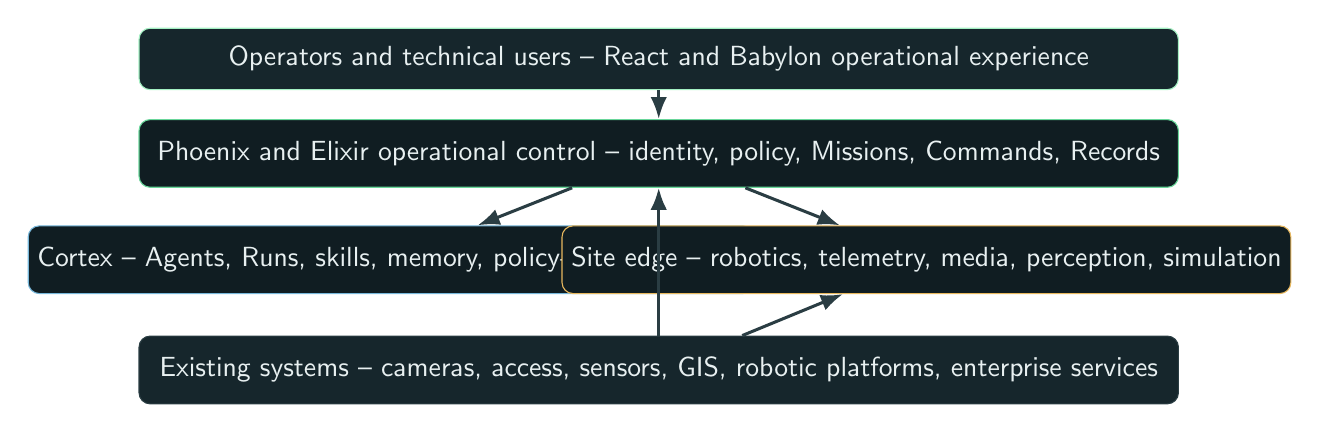
\begin{tikzpicture}[x=1cm,y=1cm]
\node[draw=mint,fill=active,text=text,rounded corners,minimum width=13.2cm,minimum height=.78cm] (u) at (6.6,5.1){Operators and technical users -- React and Babylon operational experience};
\node[draw=green,fill=panel,text=text,rounded corners,minimum width=13.2cm,minimum height=.86cm] (c) at (6.6,3.9){Phoenix and Elixir operational control -- identity, policy, Missions, Commands, Records};
\node[draw=blue,fill=panel,text=text,rounded corners,minimum width=6.1cm,minimum height=.86cm] (x) at (3.2,2.55){Cortex -- Agents, Runs, skills, memory, policy-bounded intent};
\node[draw=amber,fill=panel,text=text,rounded corners,minimum width=6.1cm,minimum height=.86cm] (e) at (10,2.55){Site edge -- robotics, telemetry, media, perception, simulation};
\node[draw=line,fill=active,text=text,rounded corners,minimum width=13.2cm,minimum height=.86cm] (s) at (6.6,1.15){Existing systems -- cameras, access, sensors, GIS, robotic platforms, enterprise services};
\draw[-{Latex},line,line width=1.1pt] (u)--(c);\draw[-{Latex},line,line width=1.1pt] (c)--(x);\draw[-{Latex},line,line width=1.1pt] (c)--(e);\draw[-{Latex},line,line width=1.1pt] (s)--(c);\draw[-{Latex},line,line width=1.1pt] (s)--(e);
\end{tikzpicture}}
\vspace{2mm}
\begin{block}{Recommended baseline}\centering Site-local operational continuity with central enterprise coordination. Existing systems remain authoritative for the facts and controls they own.\end{block}
\end{frame}

\begin{frame}{One authority path. Deliberate technical boundaries.}
\begin{columns}[T]
\column{.49\textwidth}
\begin{block}{Operational control plane owns}\small Organization and Site identity; Operations; policy; Mission and Task lifecycle; resource reservation; Command admission; evidence relationships; audit; public interfaces.\end{block}
\begin{block}{Site and edge own}\small Vendor protocols; target execution; local rejection and failsafes; high-rate telemetry; media; perception; simulation; measured native workloads.\end{block}
\column{.48\textwidth}
\begin{block}{Cortex owns}\small Agent identity and replaceable Runs; provider supervision; bounded tools; assessment; recommendations; memory retrieval; policy-permitted intent; structured requests.\end{block}
\begin{block}{Paths that do not exist}\small Browser, scheduler, or Cortex directly operating a platform; simulation identity becoming physical execution; adapters creating Mission authority; client state becoming operational truth.\end{block}
\end{columns}
\vspace{2mm}
\begin{block}{Constitution}\centering Every effect-capable human, schedule, Cortex, policy, Agent, or tool request enters the same BEAM-owned admission path.\end{block}
\end{frame}

\begin{frame}{Resilient Site cells with enterprise coordination}
\begin{columns}[T]
\column{.48\textwidth}
\begin{block}{SITE-LOCAL HELIOS}\small\begin{itemize}\item Local operator access and durable state.\item Current operational world and approved Missions.\item Site Cortex and bounded local policy.\item Robotics, telemetry, media, and perception.\item Evidence buffering and local observability.\item Bounded operation during enterprise disconnection.\end{itemize}\end{block}
\column{.48\textwidth}
\begin{block}{ENTERPRISE HELIOS}\small\begin{itemize}\item Multi-Site posture and Attention.\item Organization policy and administration.\item Central Cortex and longer-horizon analysis.\item Cross-Site requests and resource coordination.\item Federated Records, memory, and learning.\item Approved package and policy distribution.\end{itemize}\end{block}
\end{columns}
\vspace{2mm}
\centering

\begin{tikzpicture}[x=1cm,y=1cm]
\node[draw=green,fill=panel,text=text,rounded corners,minimum width=3.8cm,minimum height=.72cm] (a) at (3,0){Site A};
\node[draw=blue,fill=panel,text=text,rounded corners,minimum width=3.8cm,minimum height=.72cm] (b) at (11,0){Enterprise};
\draw[mint,line width=2pt] (a)--(b);
\node[fill=bg,text=muted,font=\scriptsize] at (7,.28){bounded, attributable federation};
\end{tikzpicture}
\vfill{\color{amber}\small Disconnection never creates new authority. Reconnect reconciles existing facts and never duplicates effects.}
\end{frame}

\begin{frame}{The operational world is authoritative context}
\begin{columns}[T]
\column{.44\textwidth}
\begin{block}{World Revision}\small Source digests; geometry; coordinate frames; transforms; calibration; uncertainty; semantic objects; zones; routes; sensors; deployments; limitations; publication and commissioning state.\end{block}
\begin{block}{Presentation package}\small Babylon or another approved renderer consumes a derived package. Presentation may be optimized; authority cannot move into the renderer.\end{block}
\column{.53\textwidth}
\centering
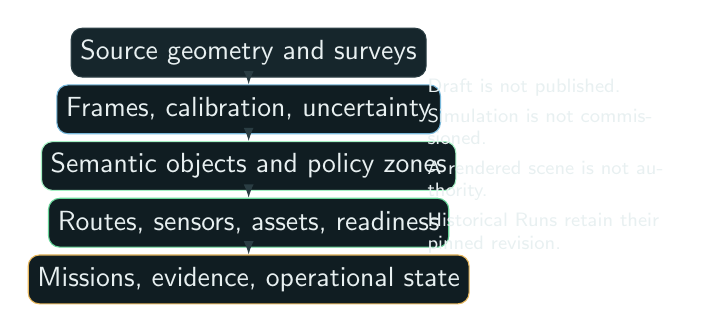
\begin{tikzpicture}[x=.78cm,y=.72cm]
\node[draw=line,fill=active,text=text,rounded corners,minimum width=3.6cm,minimum height=.62cm] (g) at (2.1,5){Source geometry and surveys};
\node[draw=blue,fill=panel,text=text,rounded corners,minimum width=3.6cm,minimum height=.62cm] (f) at (2.1,4){Frames, calibration, uncertainty};
\node[draw=mint,fill=panel,text=text,rounded corners,minimum width=3.6cm,minimum height=.62cm] (m) at (2.1,3){Semantic objects and policy zones};
\node[draw=green,fill=panel,text=text,rounded corners,minimum width=3.6cm,minimum height=.62cm] (r) at (2.1,2){Routes, sensors, assets, readiness};
\node[draw=amber,fill=panel,text=text,rounded corners,minimum width=3.6cm,minimum height=.62cm] (o) at (2.1,1){Missions, evidence, operational state};
\draw[-{Latex},line] (g)--(f);\draw[-{Latex},line] (f)--(m);\draw[-{Latex},line] (m)--(r);\draw[-{Latex},line] (r)--(o);
\node[text=text,font=\scriptsize,align=left,text width=3.1cm] at (7,3){Draft is not published.\par\vspace{1mm}Simulation is not commissioned.\par\vspace{1mm}A rendered scene is not authority.\par\vspace{1mm}Historical Runs retain their pinned revision.};
\end{tikzpicture}
\end{columns}
\end{frame}

\begin{frame}{Mission and Command: intent to observed effect}
\centering
\resizebox{.94\linewidth}{!}{%

\begin{tikzpicture}[x=1cm,y=1cm]
\node[draw=mint,fill=panel,text=text,rounded corners,minimum width=1.7cm,minimum height=.72cm] (i) at (.8,0){Intent};
\node[draw=blue,fill=panel,text=text,rounded corners,minimum width=1.9cm,minimum height=.72cm] (p) at (3.1,0){Policy};
\node[draw=amber,fill=panel,text=text,rounded corners,minimum width=2.2cm,minimum height=.72cm] (r) at (5.9,0){Readiness};
\node[draw=green,fill=panel,text=text,rounded corners,minimum width=2.1cm,minimum height=.72cm] (c) at (8.7,0){Command};
\node[draw=line,fill=active,text=text,rounded corners,minimum width=2.3cm,minimum height=.72cm] (e) at (11.6,0){Private edge};
\node[draw=mint,fill=panel,text=text,rounded corners,minimum width=1.9cm,minimum height=.72cm] (o) at (14.3,0){Observed};
\draw[-{Latex},line] (i)--(p);\draw[-{Latex},line] (p)--(r);\draw[-{Latex},line] (r)--(c);\draw[-{Latex},line] (c)--(e);\draw[-{Latex},line] (e)--(o);
\end{tikzpicture}}
\vspace{5mm}
\begin{columns}[T]
\column{.48\textwidth}
\begin{block}{Mission structure}\small Reusable Definition; immutable Revision; exact Proposal; target preparation; authorization snapshot; one admitted Run; independent Task Runs; attributable completion and Record.\end{block}
\column{.48\textwidth}
\begin{block}{Command truth is orthogonal}\small Authority, delivery, target acceptance, observed effect, and Mission consequence remain separate. One dimension cannot silently advance another.\end{block}
\end{columns}
\vspace{3mm}
\begin{block}{Unknown result}\centering If a Command may have reached a target but the response is lost, Helios reconciles that attempt. It does not blindly issue another effect.\end{block}
\end{frame}

\begin{frame}{Why sent is not the same as happened}
\centering
\resizebox{.92\linewidth}{!}{%

\begin{tikzpicture}[x=1cm,y=1cm]
\node[draw=green,fill=panel,text=text,rounded corners,minimum width=2.1cm,minimum height=.72cm] (a) at (1,0){Authorized};
\node[draw=blue,fill=panel,text=text,rounded corners,minimum width=2.1cm,minimum height=.72cm] (d) at (4,0){Delivered};
\node[draw=mint,fill=panel,text=text,rounded corners,minimum width=2.3cm,minimum height=.72cm] (t) at (7,0){Target accepted};
\node[draw=amber,fill=panel,text=text,rounded corners,minimum width=2.3cm,minimum height=.72cm] (e) at (10.2,0){Effect observed};
\node[draw=line,fill=active,text=text,rounded corners,minimum width=2.2cm,minimum height=.72cm] (o) at (13.4,0){Outcome known};
\draw[-{Latex},line] (a)--(d);\draw[-{Latex},line] (d)--(t);\draw[-{Latex},line] (t)--(e);\draw[-{Latex},line] (e)--(o);
\end{tikzpicture}}
\vspace{6mm}
\begin{columns}[T]
\column{.31\textwidth}
\begin{block}{No blind replay}\small A lost response does not create permission to issue another physical effect.\end{block}
\column{.31\textwidth}
\begin{block}{One current controller}\small Operator, Cortex Run, Site process, and edge execution obey current generation or lease authority.\end{block}
\column{.31\textwidth}
\begin{block}{Record what was known}\small Intent, authority, delivery, acceptance, effect, uncertainty, intervention, and outcome remain attributable.\end{block}
\end{columns}
\vspace{4mm}
{\color{muted}\small A missing receipt remains unknown. A stale controller is fenced. Reconnect reconciles the original attempt.}
\end{frame}

\begin{frame}{Cortex: hybrid intelligence with fenced Runs}
\begin{columns}[T]
\column{.46\textwidth}
\begin{block}{Durable Agent}\small Accountable identity, role, scope, profile revision, authority ceiling, skill and tool policy, memory scope, and human supervisor.\end{block}
\begin{block}{Replaceable Agent Run}\small Generation, provider, approved context, skills, tools, budget, audience, consequence class, checkpoint, and lease. A newer generation fences an older Run.\end{block}
\column{.51\textwidth}
\centering
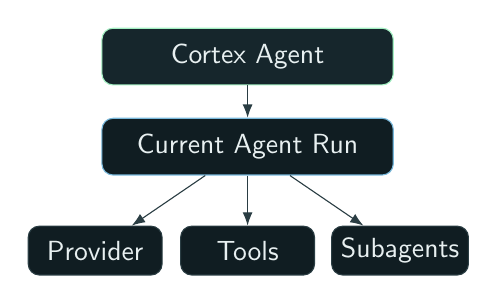
\begin{tikzpicture}[x=.88cm,y=.88cm]
\node[draw=mint,fill=active,text=text,rounded corners,minimum width=3.7cm,minimum height=.72cm] (a) at (3,4.3){Cortex Agent};
\node[draw=blue,fill=panel,text=text,rounded corners,minimum width=3.7cm,minimum height=.72cm] (r) at (3,3){Current Agent Run};
\node[draw=line,fill=panel,text=text,rounded corners,minimum width=1.7cm,minimum height=.62cm] (pr) at (.8,1.5){Provider};
\node[draw=line,fill=panel,text=text,rounded corners,minimum width=1.7cm,minimum height=.62cm] (t) at (3,1.5){Tools};
\node[draw=line,fill=panel,text=text,rounded corners,minimum width=1.7cm,minimum height=.62cm] (s) at (5.2,1.5){Subagents};
\draw[-{Latex},line] (a)--(r);\draw[-{Latex},line] (r)--(pr);\draw[-{Latex},line] (r)--(t);\draw[-{Latex},line] (r)--(s);
\end{tikzpicture}
\end{columns}
\vspace{3mm}
\begin{block}{Phase 3 autonomy}\centering Current policy + evidence + exact Site and Mission class + readiness + eligible resources + preserved reserve coverage $\rightarrow$ ordinary Mission and Command admission $\rightarrow$ operator supervision.\end{block}
\end{frame}

\begin{frame}{Media, integration, identity, and trust}
\begin{columns}[T]
\column{.49\textwidth}
\begin{block}{Media and perception}\small Camera or sensor $\rightarrow$ Site ingest $\rightarrow$ selected viewing and source-authoritative recording. Perception produces attributable detections, Tracks, observations, confidence, and provenance.\end{block}
\begin{block}{Cortex input}\small Structured semantic output, approved stills or clips, evidence references, source health, spatial context, uncertainty, and policy. Continuous raw video stays in the media path.\end{block}
\column{.48\textwidth}
\begin{block}{Integration patterns}\small Attributable events; snapshot plus delta; bounded source query; media reference; native command boundary; evidence export. Clients reload authoritative projections after gaps.\end{block}
\begin{block}{Identity and trust}\small Human, service, device, and Agent identities remain distinct. Service communication is mutually authenticated and encrypted. Browsers and model providers never receive reusable source or platform secrets.\end{block}
\end{columns}
\vspace{2mm}
\begin{block}{Evidence rule}\centering Reading, detection, Track, observation, association, Alert, Incident, evidence, assessment, recommendation, decision, Command, and outcome remain distinct attributable facts.\end{block}
\end{frame}

\begin{frame}{Degraded operation, delivery, and status}
\begin{columns}[T]
\column{.48\textwidth}
\begin{block}{Failure behavior}\small\begin{itemize}\item Source or media outage: unavailable with freshness; no negative inference.\item Cortex outage: native operator controls remain.\item Driver outage: resource degrades or becomes unavailable.\item Enterprise outage: bounded Site-local operation continues.\item Authority uncertainty: writes fail closed.\item Unknown effect: reconcile; never blind replay.\end{itemize}\end{block}
\column{.48\textwidth}
\begin{block}{Visible delivery path}\small Foundation: identity, event, mode, and no-bypass controls.\par\vspace{1mm}Phase 1: operator-directed robotic Mission and Exercise.\par\vspace{1mm}Phase 2: Cortex assessment, recommendations, memory, learning.\par\vspace{1mm}Phase 3: policy-bounded autonomous observation.\par\vspace{1mm}Phase 4: multi-Agent and cross-Site coordination.\end{block}
\end{columns}
\vspace{2mm}
\begin{block}{Current technical posture}\centering \tagcurrent\ Foundations \quad \tagdev\ Mission, Command, readiness, edge, operational Cortex \quad \tagplanned\ Federation, autonomy, memory, learning, coordination\end{block}
\vspace{2mm}
{\color{muted}\scriptsize This overview withholds implementation-ready schemas, API inventories, database definitions, exact recovery logic, Site-specific network details, operational procedures, and proprietary source structure.}
\end{frame}

\end{document}
